\documentclass{vie16}
\usepackage{wrapfig}
\usepackage{float}
\usepackage{amsmath}
\usepackage[table,xcdraw]{xcolor}
\usepackage{booktabs}
\usepackage{multirow}
\usepackage{adjustbox}

% Path to figures
\graphicspath{{Fig/}}

% COMENTAR ANTES DE SUBMETER!
% Comando temporarios
\usepackage{color}
\usepackage[normalem]{ulem}
\newcommand{\new}[1]{\textcolor{blue}{#1}}
\newcommand{\old}[1]{\textcolor{MyDarkViolet}{\sout{#1}}}
\newcommand{\att}[1]{\textcolor{red}{#1}}
\newcommand{\js}[1]{\textcolor{darkgreen}{#1}}
\newcommand{\obs}[1]{\textcolor{orange}{#1}}
\definecolor{MyDarkViolet}{rgb}{0.602,0,0.602}
\definecolor{orange}{RGB}{255,127,0}
\definecolor{darkgreen}{RGB}{0,127,0}

% For pdf hyperlinks
\usepackage{hyperref}
\hypersetup{colorlinks=true}
\hypersetup{citecolor=blue}
\hypersetup{pdftitle={Development of lock-in resistivimeter
for measuring resistivity and induced polarization under
high electrical noise}}
\hypersetup{pdfauthor={J.~M.~Oliveira and F.~Hiodo}}
% For making a print without color links
\hypersetup{linkcolor=black,citecolor=black,filecolor=black,urlcolor=black}
\hypersetup{linkcolor=blue,citecolor=blue,filecolor=blue,urlcolor=blue}
\usepackage{url}
\begin{document}

\title{Development of lock-in resistivimeter for measuring
resistivity and induced polarization under high electrical noise}
\author{J.~M.~Oliveira and F.~Hiodo}
\maketitle

% Nota: geralmente a EAGE limita o numero de caracteres no abstract. 

\begin{abstract}

	The Cole-Cole RC circuit model and the reduced clay model were
	tested with three levels of white noise in order to develop a low
	cost lock-in resistivimeter. The device has maximum power of 60
	watts and showed reliable stability under $67 \%$ and $11 \%$ of
	white noise in the respective models. The equipment was made with
	low cost components and yet capable of providing a frequency sweep
	from $13$ to $120$Hz to the transmitter which allows better signal
	sampling. This frequency bandwidth was used to find the less time
	consuming operational settings able to recover the Cole-Cole
	exponent and relaxation time, in other words, which are the minimum
	number of frequency samples that is necessary to reconstruct the
	Cole-Cole curve. An inversion scheme based on the partial sweep of
	the solution space was implemented in OCTAVE. We found that $8$
	frequency samples evenly spaced are enough to recover the relaxation
	time with variations below one order of magnitude. Therefore, the
	results showed good performance for the developed lock-in
	resistivimeter. The suggested applications to such equipment is not
	only restricted to field measurements but also to lab samples
	studies related to Spectral Induced Polarization (SIP), resistivity
	and Induced Polarization (IP) under high electrical noise.  
\end{abstract}	
		

\newpage


\section{Introduction}
Urban regions are characterized by a high noise content to the
geoelectrical methods mainly due to presence of power supply,
grounding and stray voltages. It's also known that intrusive methods
are affected by pavimentation and buildings which impose restrains in
the superficial area making them more susceptible to noise. The
objectives of this work is the design of a synchronous detection
resistivimeter from low cost components to conduct resistivity and IP
surveys using low power supply.  As observed in Figure 1 the equipment
basically consists of a transmitter and a receiver with two channels
each. The reference channel is fed directly in the receiver while the
signal channel is injected from the transmitter into the subsurface
and then to the receiver. An ideal lock-in transmitter would have an
infinite frequency sweep without any distortion and would deliver
constant power for all frequencies. However, due to physical
limitation our transmitter is capable to provide a stable power supply
close to 60W for the frequency bandwidth of 13 to 120Hz with minimal
distortion.  Bellow the 13Hz threshold the electrical sine wave
distortion increases drastically and above the 120Hz there is little
gain of information due to logarithmic nature of frequency.

\section{Sincronous Detection}
The synchronous detection also known as \textit{lock-in} is sensitive
to the difference of frequency and phase between the two inputs
\att{PRECISA DE UMA REFERENCIA AQUI}, reaching a peak when the
correlation in the frequency domain is maximum. For this reason it can
track signals with the same characteristics of the reference channel
even under intense noise since the noise doesn't have a correlated
phase \att{REFERENCIA}. Inside the receiver, the reference channel is
convert to a unitary square wave then is multiplied by the demodulated
signal as showed in the complete scheme in Figure \ref{f:Lock-in}. The
resulting DC voltage on the display is the output of the low-pass
filter of frequency no greater than the input wave as the equation
(\att{Adiciona a qeuacao}) describes 
  
Therefore, analizing the equation (\att{equacao acima}) we note two
special cases; (1) the output will be proportional only to the
resistivity if the two inputs are in phase; (2) the output will be
proportional only to the imaginary resistivity if they are in
quadrature which is related to polarization effects.

\begin{figure}[h!]
	\centering
	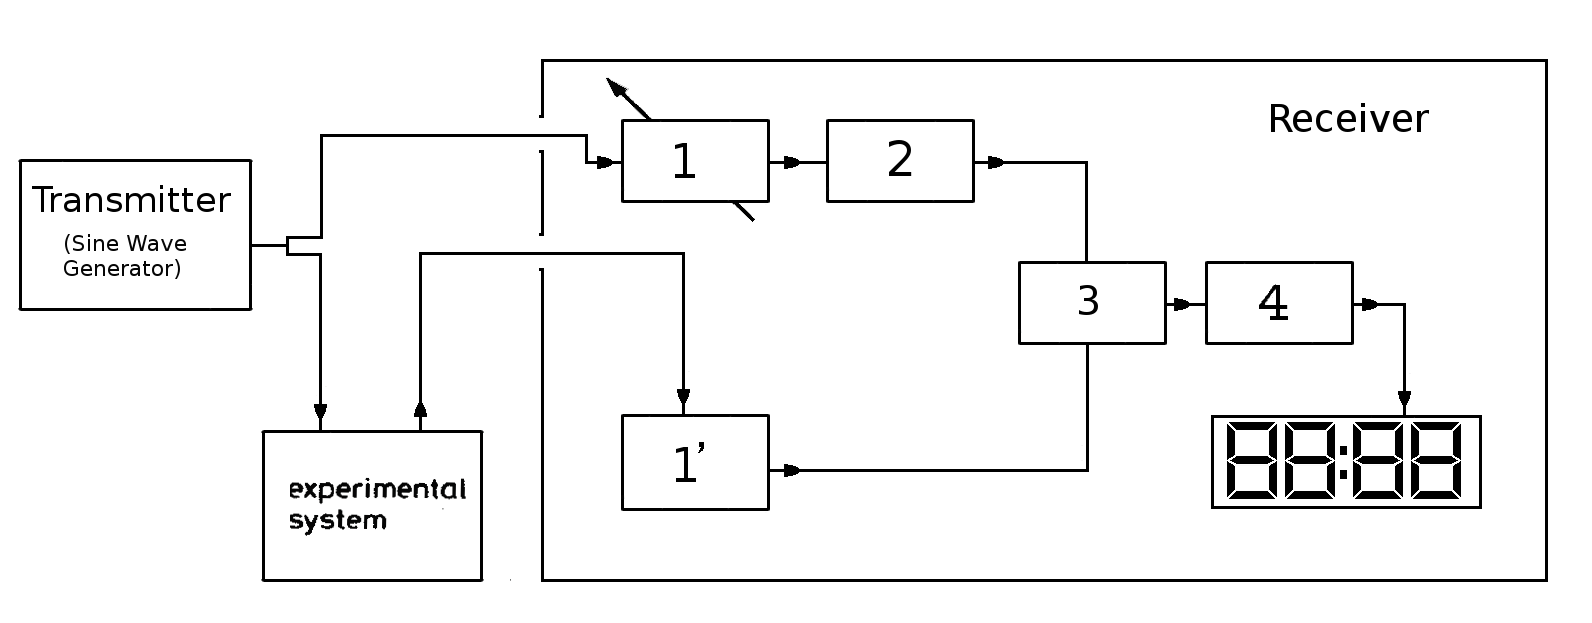
\includegraphics[keepaspectratio=true,scale=0.3]{Sistema-Inside_Lock_In}
	\caption{Scheme of synchronous detection. The arrows show the way followed by the source signal from the transmitter injected into the receiver reference channel (\textit{Up}) and signal channel (\textit{down}). In the reference channel $1^{,}$ is a optional attenuater%o que atenua. Não sei se essa palavra existe
	 . In the reference channel $1$ is a phase-shifter for correcting the added phase from the detector, $2$ output a square wave from the sine wave input, $3$ is the multiplier and  $4$ the low-pass filter led to the display. }
	\label{f:Lock-in}
\end{figure}
%imaginary resistivity pode ser electric permittivity, NÃO REMOVA ESSE PERCENT!

% Figura sistema
% transfer function do equipamento




% synchronous detection baixa deriva termica, experimento
% durou horas
\section{Scaled Models}


\section{Inversion}

As mentioned before, due to pratical limitations our resistivimeter frequency range from $13$ to $120$Hz.
While a conventional chargeability survey uses much lower frequencies, sample measurements uses higher % Como resultado a cargabilidade não bate, mas tudo bem, isso nao precisa falar... =D
so is reasonable to assume the validity of it's frequency band for application of equation \ref{e:FE}. However
find the relaxation time dor SIP survey could be %comprometido, incapacitado, algo assim
for these frequencies.


\begin{equation}
	F_{e} = \frac{ |V_{(\omega_{1})} - V_{(\omega_{2})}| }{V_{(\omega_{1})}}
	\label{e:FE}
\end{equation}


To study this application we made a inversion of Cole-Cole parameters using the frequencies
at range of our resistivimeter only. The inverted parameters were the relaxation time and exponent
from equation \ref{e:CC}. In the equation $\sigma_{e}$ is the complex conductivity, $\sigma_{0}$ is the
conductivity at zero frequency, $m$ is the chargeability, $\omega$ is the angular frequency, $\tau$ is the relaxation time
and $c$ is the Cole-Cole exponent.

\begin{equation}
	\sigma_{e} = \sigma_{0}
			\left[
			1 + \frac{m}{1-m}
						\left( 
								1 - \frac{1}{1+ \left( j\omega\tau \right)^{c} }	
						\right) 			
			\right]
	\label{e:CC}
\end{equation}

The case in analysis were for one relaxation time only. It was tested for four values of Gaussian noise and 
for four different frequency sampling at $5\%$ of noise.


\section{Results}


\begin{table}[h!]
\centering
\caption{Measured voltage on scaled models with three levels of white noise.}
\label{t:scaled_models}
\begin{tabular}{cccl|ccc}
\multirow{2}{*}{\textbf{Noise level (\%)}}  & \multicolumn{2}{c}{\textbf{Output}}     &  & \textbf{Noise Level (\%)} & \multicolumn{2}{c}{\textbf{Output}}     \\
                         & \textbf{In Phase}  & \textbf{Quadrature} &  &  	 				& \textbf{In Phase} & \textbf{Quadrature} 	\\
\multirow{4}{*}{0}	 		& 1.52              & 8.45                &  & 	\multirow{4}{*}{0}	&  5.24				&		1.80			\\
					 		& 1.60              & 8.50                &  &						&  4.75				&		1.90			\\
					 		& 1.44              & 8.46                &  &						&  4.80				&		1.92			\\
					 		& 1.48              & 8.40                &  &						&  5.30		    	&		1.81	 
                                         \\ \hline                                   
\multirow{4}{*}{40}	 		& 1.06              & 8.42                &  & 	\multirow{4}{*}{11}	&	4.70			&		1.32			\\
					 		& 1.28              & 8.41                &  &						&	4.60			&		1.20			\\
					 		& 1.29              & 8.37                &  &						&	4.68			&		1.26			\\
					 		& 1.30              & 8.45                &  &						&	4.50			&		1.28			  
                                         \\ \hline
\multirow{4}{*}{67}	 		& 1.29              & 8.48                &  & 	\multirow{4}{*}{27}	&	2.30			&		1.30			\\
					 		& 1.28              & 8.48                &  &						&	2.05			&		1.20			\\
					 		& 1.29              & 8.48                &  &						&	2.12			&		1.24			\\
					 		& 1.30              & 8.50                &  &						&	2.50			&		1.32			  
                                          \\ \hline
\end{tabular}
\end{table}


\begin{table}[h!]
\centering
\caption{Sampling effect on the inversion of Cole-Cole parameters}
\label{my-label}
\begin{tabular}{@{}|c|c|c|c|c|c|c|c|@{}}
\multicolumn{3}{|c|}{\textbf{Sinthetic Model}}                             & \multirow{2}{*}{\textbf{Sampling}} & \multicolumn{3}{c|}{\textbf{Calculated Model}}                          & \multirow{2}{*}{\textbf{Missfit}}    \\
\textbf{Model}     & \textbf{$\tau$}          & \textbf{$e_{cc}$}          &                                    & \textbf{$\tau$} & \textbf{$e_{cc}$} & \textbf{$\tau$ deviation}         &                                      \\ \hline
\multirow{4}{*}{A} & \multirow{4}{*}{567.243} & \multirow{4}{*}{0.0452261} & 2                                  & 517.092         & 0.045(1)          & 113 \textless$\tau$\textless 1702 & 0.02                                 \\
                   &                          &                            & 4                                  & 474.313         & 0.045(1)          & 454 \textless$\tau$\textless 1702 & 0.01                                 \\
                   &                          &                            & 8                                  & 567.243         & 0.0452261         & 568 \textless$\tau$\textless 850  & 0.02                                 \\
                   &                          &                            & 16                                 & 517.092         & 0.045(1)          & 453 \textless$\tau$\textless 568  & 0.03                                 \\ \hline
\multirow{4}{*}{B} & \multirow{4}{*}{2.89942} & \multirow{4}{*}{0.0452261} & 2                                  & 2.89942         & 0.045(1)          & 0.5 \textless$\tau$\textless 2.9  & 0.007                                \\
                   &                          &                            & 4                                  & 2.89942         & 0.045(1)          & 0.5 \textless$\tau$\textless 2.9  & 0.013                                \\
                   &                          &                            & 8                                  & 2.89942         & 0.045(1)          & 1.5 \textless$\tau$\textless 11.6 & 0.015                                \\
                   &                          &                            & 16                                 & 2.89942         & 0.0452261         & 2.3 \textless$\tau$\textless 2.9  & \textless $10^{-5}$                  \\ \hline
\multirow{4}{*}{C} & \multirow{4}{*}{622.257} & \multirow{4}{*}{0.834171}  & 2                                  & 622.257         & 0.834171          & 622.257                           & \multirow{4}{*}{\textless $10^{-5}$} \\
                   &                          &                            & 4                                  & 622.257         & 0.834171          & 622.257                           &                                      \\
                   &                          &                            & 8                                  & 622.257         & 0.834171          & 622.257                           &                                      \\
                   &                          &                            & 16                                 & 622.257         & 0.834171          & 622.257                           &                                   \\  \hline
\end{tabular}
\end{table}



\begin{table}[h!]
\centering
\caption{Noise effect on the inversion of Cole-Cole parameters}
\label{my-label}
\begin{tabular}{@{}|c|c|c|c|c|c|c|@{}}
\multicolumn{3}{|c|}{\textbf{Sinthetic Model}}                             & \multirow{2}{*}{\textbf{\begin{tabular}[c]{@{}c@{}}Noise\\ (\%)\end{tabular}}} & \multicolumn{3}{c|}{\textbf{Calculated Model}}                            \\
\textbf{Model}     & \textbf{$\tau$}          & \textbf{$e_{cc}$}          &                                                                                & \textbf{$\tau$} & \textbf{$e_{cc}$} & \textbf{$\tau$ deviation}           \\  \hline
\multirow{4}{*}{A} & \multirow{4}{*}{567.243} & \multirow{4}{*}{0.0452261} & 5                                                                              & 567.243         & 0.0452261         & 567 \textless$\tau$\textless 860    \\
                   &                          &                            & 10                                                                             & 517.092         & 0.0452(5)         & 113 \textless$\tau$\textless 3405   \\
                   &                          &                            & 25                                                                             & 517.092         & 0.045(1)          & 56 \textless$\tau$\textless 5670    \\
                   &                          &                            & 250                                                                            & 517.092         & 0.045(2)          & 170 \textless$\tau$\textless 11344  \\ \hline
\multirow{4}{*}{B} & \multirow{4}{*}{2.89942} & \multirow{4}{*}{0.0452261} & 5                                                                              & 2.89942         & 0.0452(5)         & 1.15 \textless$\tau$\textless 11.6  \\
                   &                          &                            & 10                                                                             & 2.89942         & 0.045(1)          & 2.3 \textless$\tau$\textless 4.4    \\
                   &                          &                            & 25                                                                             & 2.89942         & 0.045(5)          & 1.8 \textless$\tau$\textless 5.8    \\
                   &                          &                            & 250                                                                            & 2.89942         & 0.04(1)           & 1.8 \textless$\tau$\textless 14500  \\ \hline
\multirow{4}{*}{C} & \multirow{4}{*}{622.257} & \multirow{4}{*}{0.834171}  & 5                                                                              & 622.257         & 0.834171          & 622.257                             \\
                   &                          &                            & 10                                                                             & 622.257         & 0.834171          & 622.257                             \\
                   &                          &                            & 25                                                                             &                 &                   &                                     \\
                   &                          &                            & 250                                                                            & 622.257         & 0.8(1)            & 435 \textless $\tau $\textless 1245
\end{tabular}
\end{table}



\section{Conclusions}

In relation to others instruments in use, our low power resistivimeter is able to reject great amount of noise in scaled models, returning stable measures with levels of white noise of $67 \%$ in RC circuit and $11 \%$ in clay scaled model. This results strongly support the viabilty of such low cost device in geoelectrical measures, even in noise environments.

The inversion of Cole-Cole parameters: relaxation time and Cole-Cole expoent points towards application as a multifrequency resistivimeter for Spectral Induced Polarization with a bandwith of $13$ to $120$ Hertz. In this specter $8$ points evenly distributed were enough to recover the Cole-Cole parameters.



%A  intensa rejei\c{c}\~ao de ru\'idos pelo m\'etodo de detec\c{c}\~ao s\'incrona permite a manufatura de eletrorresistiv\'imetros com baixo custo de mercado e baixa pot\^encia de opera\c{c}\~ao se comparado a outros equipamentos em uso no mercado. 
		
%		Este tipo de eletrorresistiv\'imetro apresentou estabilidade para at\'e $11\%$ de ru\'ido branco para as medidas da argila no modelo em escala reduzida. Este nivel de ru\'ido representa uma situa\c{c}\~ao muito desfavor\'avel para a aquisi\c{c}\~ao geoel\'etrica, mostrando que o desempenho do equipamento \'e suficientemente confi\'avel para sua aplica\c{c}\~ao em ambientes ruidosos.
		
%		Dada a possibilidade de aquisi\c{c}\~ao com v\'arias frequ\^encias, foi analisado o potencial da aplica\c{c}\~ao do eletrorresisitiv\'imetro na medida de polariza\c{c}\~ao ind\'uzida espectral. Os resultados obtidos pela invers\~ao dos par\^ametro de Cole-Cole, sugerem que a faixa de $13$ a $110$ Hertz \'e suficiente para a recupera\c{c}\~ao dos par\^ametros do modelo.
		
%		De maneira a aperfei\c{c}oar o equipamento para uso em campo, \'e sugerido a digitaliza\c{c}\~ao da sa\'ida, desta forma a fase poderia ser medida diretamente no equipamento eliminando a etapa de calibra\c{c}\~ao. Esta medida tamb\'em que os dados sejam salvos no equipamento, acelerando o seu processamento. 
\section{Acknowledgements (Optional)}

This is the first sentence of the acknowledgements.

% \begin{thebibliography}{6pt}
%   \bibitem[{<reference>}]{<cite>} ...
% \end{thebibliography}
%
% or
%
% \bibliography{...}

\end{document} 